\chapter{Specifikacija programske potpore}

\section{Funkcionalni zahtjevi}

\textbf{\textit{dio 1. revizije}}\\

%\textit{Navesti \textbf{dionike} koji imaju \textbf{interes u ovom sustavu} ili  \textbf{su nositelji odgovornosti}. To su prije svega korisnici, ali i administratori sustava, naručitelji, razvojni tim.}\\

%\textit{Navesti \textbf{aktore} koji izravno \textbf{koriste} ili \textbf{komuniciraju sa sustavom}. Oni mogu imati inicijatorsku ulogu, tj. započinju određene procese u sustavu ili samo sudioničku ulogu, tj. obavljaju određeni posao. Za svakog aktora navesti funkcionalne zahtjeve koji se na njega odnose.}\\


\noindent \textbf{Dionici:}

\begin{packed_enum}
	
	\item Administrator
	\item Kartograf			
	\item Igrač/korisnik	
	\item Neregistrirani/neprijavljeni korisnik
	\item Baza podataka - U primjeru dokumentacije nije navedena
	\item Razvojni tim
	
	
\end{packed_enum}

\noindent \textbf{Aktori i njihovi funkcionalni zahtjevi:}


\begin{packed_enum}
	\item  \underbar{Neregistrirani/neprijavljeni korisnik(inicijator) može se:}
	
	\begin{packed_enum}
		
		\item registrirati u sustav, stvoriti novi korisnički račun za koji su mu potrebni korisničko ime,
		fotografija, lozinka, email adresa i lokacija uređaja.
		\begin{packed_enum}
			
			\item  ukoliko se korisnik želi registrirati kao kartograf potrebno je dodati IBAN i fotografiju osobne
			
		\end{packed_enum}
		
	\end{packed_enum}
	
	\item  \underbar{Igrač (inicijator) može:}
	
	\begin{packed_enum}
		
		\item pregledati profil drugih igrača(ime, sakupljene karte, rang, winrate, statistiku zadnih 10 borbi)
		
		\item mijenjati i pregledati svoje osobne podatke 
		
		\item sakupiti kartu ulaskom u određeni radijus stvarne lokacije
		
		\item pregledati ostale igrače unutar 50km
		\begin{packed_enum}
			
			\item moguće poslati zahtjev za borbu dostupnim igračima
			
		\end{packed_enum}
		
		\item pregledati stvarnu mapu i svoju poziciju ---  \textit{google-ova ili slično} 
		
		\item pregledati naziv, opis, fotografiju i jačinu karte iz preglednika stvarne mape(pop out)
		
		\item prijaviti željenu lokaciju u blizini i ispuniti atribute
		
		\item pregledati globalnu statistiku odigranih borbi
		
		\item pregledati globalnu statistiku sakupljenih karata
		
		\item pregledati elo poredak svih igrača
		
		\item birati karte za špil koji se koristi u borbama
		
		
	\end{packed_enum}
	\item  \underbar{Kartograf (inicijator) može:}
	
	\begin{packed_enum}
		
		\item pregledati sve prijavljene lokacije
		
		\item potvrditi, odbiti i urediti prijavljene lokacije
		\begin{packed_enum}
			
			\item označiti prijavljenu lokaciju za potvrdu s terena
			
		\end{packed_enum}
		
		\item odabrati koje će lokacije potvrditi s terena
		
	\end{packed_enum}
	
	\item  \underbar{Administrator (inicijator) može:}
	
	\begin{packed_enum}
		
		\item sve funkcionalnosti igrača i kartografa
		
		\item potvrditi registraciju kartografa
		
		\item privremeno isključiti igrača iz igre
		
		\item urediti postojeće lokacije(karte) u igri
		
		\item vidjeti i uređivati popis svih korisnika i njihovih osobnih podataka. 
		
	\end{packed_enum}
	
	\item  \underbar{Baza podataka (sudionik): }
	
	\begin{packed_enum}
		
		\item pohranjuje sve podatke o korisnicima i njihovim ovlastima
		
		\item pohranjuje sve podatke o lokacijama (kartama)
		
		\item  pohranjuje podatke o borbama
		
		
	\end{packed_enum}
\end{packed_enum}

\eject 



\subsection{Obrasci uporabe}

\textbf{\textit{dio 1. revizije}}

\subsubsection{Opis obrazaca uporabe}
%\textit{Funkcionalne zahtjeve razraditi u obliku obrazaca uporabe. Svaki obrazac je potrebno razraditi prema donjem predlošku. Ukoliko u nekom koraku može doći do odstupanja, potrebno je to odstupanje opisati i po mogućnosti ponuditi rješenje kojim bi se tijek obrasca vratio na osnovni tijek.}\\

\noindent \underbar{\textbf{UC1 -  Registracija kao igrač ili kao kartograf}}
\begin{packed_item}
	\item \textbf{Glavni sudionik: } Igrač, Kartograf
	\item  \textbf{Cilj:} Stvoriti korisnički račun za pristup
	\item  \textbf{Sudionici:} Baza podataka
    \item \textbf{Preduvjeti:} 
    \item[] \begin{packed_enum}
        \item Korisnik prijavljen kao igrač ili administrator
    \end{packed_enum}
	\item  \textbf{Opis osnovnog tijeka:}
	\item[] \begin{packed_enum}
	\item Odabir načina registriranja
	\item Unos korisničkih podataka u svrhu registracije
    \item Pop Up obavijest o uspješnoj registraciji
	\end{packed_enum}
	\item  \textbf{Opis mogućih odstupanja:}
	\item[] \begin{packed_enum}
	    \item Odabir već zauzetog profilnog imena i/ili e-maila. Unos neispravnog formata ili nepostojeće e-mail adrese.
        \item[] \begin{packed_enum}
        	\item Sustav obavještava korisnika o neuspjelom upisu i vraća ga na neispunjenu formu registracije za ponovni pokušaj.
            \item Korisnik mijenja potrebne podatke te uspijeva u registaciji ili od nje odustaje.
        \end{packed_enum}
	\end{packed_enum}
\end{packed_item}

\noindent \underbar{\textbf{UC2 -  Sakupljanje karata}}
\begin{packed_item}
	\item \textbf{Glavni sudionik: } Igrač ili administrator
	\item  \textbf{Cilj:} Skupljanje nove igraće karte s određene lokacije
	\item  \textbf{Sudionici:} Baza podataka
    \item \textbf{Preduvjeti:}
	\item[]  \begin{packed_enum}
	    \item Korisnik prijavljen kao igrač ili administrator
        \item Broj karata koju igrač posjeduje je manja od gornjeg limita
        \item Korisnik se nalazi na lokaciji te karte
	\end{packed_enum}
	\item  \textbf{Opis osnovnog tijeka:}
	\item[] \begin{packed_enum}
        \item Korisnik dođe do lokacije karte
        \item Korisnik odabire "Skupi kartu lokacije"
		\item Aplikacija dodjeljuje korisniku kartu
	\end{packed_enum}
	\item  \textbf{Opis mogućih odstupanja:}
	\item[] \begin{packed_enum}
	    \item Broj karata u posjedu igrača je već dosegnuo gornji limit
        \item[] \begin{packed_enum}
        	\item Sustav obavještava korisnika o neuspjelom prihvaćanju karte i vraća ga na kartu početnog zaslona
        \end{packed_enum}
	\end{packed_enum}
\end{packed_item}

\noindent \underbar{\textbf{UC3 -  Korisnik ulazi u borbu sa drugim korisnicima}}
\begin{packed_item}
	\item \textbf{Glavni sudionik:} Igrač ili administrator
	\item  \textbf{Cilj:} Borba između igrača s ciljem osvajanja ELO bodova
	\item  \textbf{Sudionici:} Baza podataka
    \item \textbf{Preduvjeti:}
	\item[]  \begin{packed_enum}
	    \item Korisnici su prijavljeni kao igrač ili administrator
        \item Drugi korisnik je udaljen od prvog do 50 km
        \item Drugi korisnik je u tom trenutku također aktivan
	\end{packed_enum}
	\item  \textbf{Opis osnovnog tijeka:}
	\item[] \begin{packed_enum}
        \item Korisniku se prikazuju profili igrača u blizini
        \item Korisnik odabire "Profil" nekog igrača
        \item Aplikacija prikazuje profil drugog igrača
        \item Korisnik odabire "Izazovi"
        \item Drugi korisnik prihvaća izazov i korisnici ulaze u borbu jedan protiv drugoga
        \item Igrač odabire kartu koju bi htio odigrati
        \item Računalo evaulira pobjednika borbe znajući jačine odigranih karata i zapisuje rezultat u bazu podataka
        \item Korisniku se prikazuje konačan ishod borbe
        \item Karti s kojom je korisnik igrao se smanjuje vrijednost
	\end{packed_enum}
	\item  \textbf{Opis mogućih odstupanja:} 
    \item[] \begin{packed_enum}
        \item Drugi korisnik je bio unutar 50 km ali je izašao u međuvremenu dok ga je korisnik pozvao na borbu
        \item Drugi korisnik je odbio izazov
    \end{packed_enum}
\end{packed_item}

\noindent \underbar{\textbf{UC4 -  Igrač može vidjeti naziv, fotografiju, opis i jačinu karte}}
\begin{packed_item}
	\item \textbf{Glavni sudionik: } Igrač ili administrator
	\item  \textbf{Cilj:} Informiranje korisnika o određenoj igračoj karti
	\item  \textbf{Sudionici:} Baza podataka
    \item \textbf{Preduvjeti:} Korisnik je prijavljen kao igrač ili administrator
	\item  \textbf{Opis osnovnog tijeka:} 
    \item[] \begin{packed_enum}
        \item Klikom miša korisnik ulazi u kartu
        \item Korisniku se prikazuje karta
    \end{packed_enum}
\end{packed_item}

\noindent \underbar{\textbf{UC5 - Prijavljivanje željene lokacije}}
\begin{packed_item}
	\item \textbf{Glavni sudionik: } Igrač ili administrator
	\item  \textbf{Cilj:} Dodati lokaciju
	\item  \textbf{Sudionici:} Baza podataka
    \item \textbf{Preduvjeti:}
	\item[]  \begin{packed_enum}
	    \item Korisnik je registriran kao igrač ili administrator
        \item Korisnik treba biti u blizini željene lokacije
        \item Igrač treba imati sakupljeno dovoljno iskustva 
	\end{packed_enum}
	\item  \textbf{Opis osnovnog tijeka:}
	\item[] \begin{packed_enum}
	\item Korisnik odabire opciju "Predloži lokaciju"
	\item Korisnik ispunjava podatke o lokaciji
	\end{packed_enum}
	\item  \textbf{Opis mogućih odstupanja:}
	\item[] \begin{packed_enum}
	    \item Korisnik predlaže lokaciju koja je već na karti označena 
	\end{packed_enum}
\end{packed_item}

\noindent \underbar{\textbf{UC6 - Pregled profila igrača}}
\begin{packed_item}
    \item \textbf{Glavni sudionik: }Igrač ili administrator
    \item \textbf{Cilj: }Pregledati profil bilo kojeg igrača
    \item \textbf{Sudionici: }Baza podataka
    \item \textbf{Preduvjet: }Korisnik registriran kao igrač ili administrator
    \item \textbf{Opis osnovnog tijeka: }
    \item[] \begin{packed_enum}
        \item Korisnik odabire profil igrača
        \item Prikazuje se profil igrača
    \end{packed_enum}
\end{packed_item}

\noindent \underbar{\textbf{UC7 - Prikaz sakupljenih karata igrača na profilu}}
\begin{packed_item}
    \item \textbf{Glavni sudionik: }Igrač ili administrator
    \item \textbf{Cilj: } Prikazati sakupljene karte igrača
    \item \textbf{Sudionici: }Baza podataka
    \item \textbf{Preduvjet: }Korisnik je registriran kao igrač ili administrator
    \item \textbf{Opis osnovnog tijeka: }
    \item[] \begin{packed_enum}
        \item Korisnik odabire profil igrača
        \item Prikazuju se sve sakupljene karte odabranog igrača 
    \end{packed_enum}
\end{packed_item}

\noindent \underbar{\textbf{UC8 - Prikaz ranga igrača na profilu}}
\begin{packed_item}
    \item \textbf{Glavni sudionik: }Igrač ili administrator
    \item \textbf{Cilj: }Pregledati rang bilo kojeg igrača
    \item \textbf{Sudionik: }Baza podataka
    \item \textbf{Preduvjet: }Korisnik je registriran kao igrač ili administrator
    \item \textbf{Opis osnovnog tijeka:}
    \item[] \begin{packed_enum}
        \item Korisnik odabire profil igrača 
        \item Prikazuje se rang odabranog igrača
    \end{packed_enum}
\end{packed_item}

\noindent \underbar{\textbf{UC9 - Prikaz statistike zadnjih 10 borbi igrača na profilu}}
\begin{packed_item}
    \item \textbf{Glavni sudionik: }Igrač ili administator
    \item \textbf{Cilj: } Pregledati zadnjih 10 borbi i njihov rezultat
    \item \textbf{Sudionici: }Baza podataka
    \item \textbf{Preduvjet: }Korisnik je registriran kao igrač ili administrator
    \item \textbf{Opis osnovnog tijeka: }
    \item[] \begin{packed_enum}
        \item Korisnik odabire profil igrača
        \item Prikazuje se zadnjih 10 borbi i njihov rezultat
    \end{packed_enum}
\end{packed_item}

\noindent \underbar{\textbf{UC10 - Prikaz globalne statistike odigranih borbi svih igrača}}
\begin{packed_item}
    \item \textbf{Glavni sudionik: }Igrač ili administrator
    \item \textbf{Cilj: }Pregledati globalnu statistiku borbi svih igrača
    \item \textbf{Sudionici: }Baza podataka
    \item \textbf{Preduvjet: }Korisnik je prijavljen kao igrač ili administrator
    \item \textbf{Opis osnovnog tijeka: }
    \item[] \begin{packed_enum}
        \item Korisnik odabire "Globalna statistika borbi"
        \item Prikazuje se globalna statistika svih odigranih borbi
    \end{packed_enum}
\end{packed_item}

\noindent \underbar{\textbf{UC11 - Prikaz globalne statistike svih lokacija}}
\begin{packed_item}
    \item \textbf{Glavni sudionik: }Igrač ili administrator
    \item \textbf{Cilj: }Pregledati globalnu statistiku lokacija
    \item \textbf{Sudionici: }Baza podataka
    \item \textbf{Preduvjet: }Korisnik je prijavljen kao igrač ili administrator
    \item \textbf{Opis osnovnog tijeka: }
    \item[] \begin{packed_enum}
        \item Korisnik odabire "Sve lokacije"
        \item Prikazuje se sve lokacije koje se nalaze u igrici
    \end{packed_enum}
\end{packed_item}

\noindent \underbar{\textbf{UC12 – Pregled poretka igrača}}
\begin{packed_item}
	
	\item \textbf{Glavni sudionik: }Igrač, Administrator
	\item  \textbf{Cilj:} Pregledati poretke svih igrača
	\item  \textbf{Sudionici:} Baza podataka
	\item  \textbf{Preduvjet:} Korisnik je već prijavljen kao igrač ili administrator
	\item  \textbf{Opis osnovnog tijeka:}
	
	\item[] \begin{packed_enum}
		
		\item Korisnik odabire opciju „Poredak igrača“
		\item Prikaže se trenutni poredak svih igrača koji je izračunat prema elo sustavu
	\end{packed_enum}
\end{packed_item}

\noindent \underbar{\textbf{UC13 – Pregled prijavljenih lokacija}}
\begin{packed_item}
	
	\item \textbf{Glavni sudionik: }Kartograf, Administrator
	\item  \textbf{Cilj:} Pregledati sve lokacije koje su igrači prijavili
	\item  \textbf{Sudionici:} Baza podataka
	\item  \textbf{Preduvjet:} Korisnik je već prijavljen kao kartograf ili administrator
	\item  \textbf{Opis osnovnog tijeka:}
	
	\item[] \begin{packed_enum}
		
		\item Korisnik u aplikaciji odabire opciju „Pregled prijavljenih lokacija“
		\item Prikaže se karta na kojoj su označene sve lokacije koje su igrači prijavili
		\item Korisnik klikne na jednu od lokacija na karti
		\item Prikazuju se podatci o lokaciji te tri opcije (potvrdi, uredi i obriši)
	\end{packed_enum}
\end{packed_item}

\noindent \underbar{\textbf{UC14 – Potvrđivanje prijavljenih lokacija}}
\begin{packed_item}
	
	\item \textbf{Glavni sudionik: }Kartograf, Administrator
	\item  \textbf{Cilj:} Prihvatiti prijavljenu lokaciju
	\item  \textbf{Sudionici:} Baza podataka
	\item  \textbf{Preduvjet:} Korisnik je već prijavljen kao kartograf ili administrator
	\item  \textbf{Opis osnovnog tijeka:}
	
	\item[] \begin{packed_enum}
		
		\item Korisnik u aplikaciji odabire opciju „Pregled prijavljenih lokacija“
		\item Prikaže se karta na kojoj su označene sve lokacije koje su igrači prijavili
		\item Korisnik klikne na jednu od lokacija na karti
		\item Korisnik odabire opciju "Potvrdi"
		\item Lokacija se u bazi podataka označuje kao potvrđena
		\item Lokacija postaje vidljiva igračima unutar aplikacije
		\item Igrač koji je prijavio lokaciju dobiva potvrđenu kartu
	\end{packed_enum}
	
	\item  \textbf{Opis mogućih odstupanja:}
	
	\item[] \begin{packed_item}
		
		\item[3.a]  U bazi nema prijavljenih lokacija
		
	\end{packed_item}
\end{packed_item}

\noindent \underbar{\textbf{UC15 – Uređivanje prijavljenih lokacija}}
\begin{packed_item}
	
	\item \textbf{Glavni sudionik: }Kartograf, Administrator
	\item  \textbf{Cilj:} Urediti prijavljenu lokaciju
	\item  \textbf{Sudionici:} Baza podataka
	\item  \textbf{Preduvjet:} Korisnik je već prijavljen kao kartograf ili administrator
	\item  \textbf{Opis osnovnog tijeka:}
	
	\item[] \begin{packed_enum}
		
		\item Korisnik u aplikaciji odabire opciju „Pregled prijavljenih lokacija“
		\item Prikaže se karta na kojoj su označene sve lokacije koje su igrači prijavili
		\item Korisnik klikne na jednu od lokacija na karti
		\item Korisnik odabire opciju "Uredi"
		\item Korisnik mijenja podatke o lokaciji
		\item Korisnik klikne na gumb "Spremi promjene"
		\item Baza podataka se ažurira
	\end{packed_enum}
	
	\item  \textbf{Opis mogućih odstupanja:}
	
	\item[] \begin{packed_item}
		
		\item[3.a]  U bazi nema prijavljenih lokacija
		\item[5.a]  Korisnik nije spremio podatke
		\item[] \begin{packed_enum}
			
			\item Sustav obavještava korisnika da nije spremio podatke
			
		\end{packed_enum}
		
	\end{packed_item}
\end{packed_item}

\noindent \underbar{\textbf{UC16 – Odbijanje prijavljenih lokacija}}
\begin{packed_item}
	
	\item \textbf{Glavni sudionik: }Kartograf, Administrator
	\item  \textbf{Cilj:} Odbiti prijavljenu lokaciju
	\item  \textbf{Sudionici:} Baza podataka
	\item  \textbf{Preduvjet:} Korisnik je već prijavljen kao kartograf ili administrator
	\item  \textbf{Opis osnovnog tijeka:}
	
	\item[] \begin{packed_enum}
		
		\item Korisnik u aplikaciji odabire opciju „Pregled prijavljenih lokacija“
		\item Prikaže se karta na kojoj su označene sve lokacije koje su igrači prijavili
		\item Korisnik klikne na jednu od lokacija na karti
		\item Korisnik odabire opciju "Obriši"
		\item Lokacija se uklanja iz baze podataka
	\end{packed_enum}
	
	\item  \textbf{Opis mogućih odstupanja:}
	
	\item[] \begin{packed_item}
		
		\item[3.a]  U bazi nema prijavljenih lokacija
		
	\end{packed_item}
\end{packed_item}

\noindent \underbar{\textbf{UC17 -Pregled lokacija kojima je potrebna potvrda s terena}}
\begin{packed_item}
	
	\item \textbf{Glavni sudionik: }Kartograf, Administrator
	\item  \textbf{Cilj:} Pregled svih lokacija kojima je potrebna potvrda s terena
	\item  \textbf{Sudionici:} Baza podataka
	\item  \textbf{Preduvjet:} Korisnik je prijavljen kao kartograf ili administrator
	\item  \textbf{Opis osnovnog tijeka:}
	
	\item[] \begin{packed_enum}
		
		\item Korisnik odabire opciju "Pregled lokacija za potvrdu s terena"
		\item Prikaže se lista lokacija koje zahtijevaju potvrdu s terena
	\end{packed_enum}
\end{packed_item}


\noindent \underbar{\textbf{UC18 - Odabiranje lokacija za osobnu potvrdu s terena}}
\begin{packed_item}
	
	\item \textbf{Glavni sudionik: }Kartograf, Administrator
	\item  \textbf{Cilj:} Označiti koje od lokacija za potvrdu s terena će korisnik osobno provjeriti
	\item  \textbf{Sudionici:} Baza podataka
	\item  \textbf{Preduvjet:} Korisnik je prijavljen kao kartograf ili administrator
	\item  \textbf{Opis osnovnog tijeka:}
	
	\item[] \begin{packed_enum}
		
		\item Korisnik odabire opciju "Pregled lokacija za potvrdu s terena"
		\item Prikaže se lista lokacija koje zahtjevaju potvrdu s terena
		\item Korisnik označava lokacije koje on želi osobno provjeriti
		\item Nakon pritiska gumba "Dohvati put", označene lokacije postanu vidljive samo tom korisniku na stranici "Pregled lokacija za potvrdu s terena"
		\item Sustav preko vanjskog servisa OSRM dohvati rješenje problema trgovačkog putnika
		\item Sustav korisniku put prikaže na karti na stranici „Pregled prijavljenih lokacija“
		\item Korisnik je preusmjeren na stranicu „Pregled prijavljenih lokacija“
	\end{packed_enum}	
	
	\item  \textbf{Opis mogućih odstupanja:}
	
	\item[] \begin{packed_item}
		
		\item[3.a] Korisnik nikad ne potvrdi lokaciju s terena
		\item[] \begin{packed_enum}
			
			\item Postaviti vremenski rok od trenutka prihvaćanja
			
		\end{packed_enum}
		\item[4.a] Korisnik ne pritisne gumb "Dohvati put" te pokuša izaći iz stranice
		\item[] \begin{packed_enum}
			
			\item Sustav obaviještava korisnika da nije spremio podatke
			
		\end{packed_enum}
		\item[4.b] Korisnik je imao prethodno označene lokacije
		\item[] \begin{packed_enum}
			
			\item Lokacije koje više nisu označene su ponovno vidljive svim korisnicima
			
		\end{packed_enum}
	\end{packed_item}
\end{packed_item}


\noindent \underbar{\textbf{UC19 -Potvrda registracije kartografa}}
\begin{packed_item}
	
	\item \textbf{Glavni sudionik: } Administrator
	\item  \textbf{Cilj:} Prihvatiti kartografa u sustav
	\item  \textbf{Sudionici:} Kartograf, Baza podataka
	\item  \textbf{Preduvjet:} Korisnik je registriran i dodijeljena su mu prava administratora
	\item  \textbf{Opis osnovnog tijeka:}
	
	\item[] \begin{packed_enum}
		
		\item Administrator odabire opciju "Pregled prijavljenih kartografa"
		\item Prikaže se lista prijavljenih kartografa s opcijama "Potvrdi" i "Odbij" pored svakog kartografa
		\item Administrator klikne na gumb "Potvrdi"
		\item Kartograf se sprema u bazu kao potvrđen
	\end{packed_enum}
\end{packed_item}

\noindent \underbar{\textbf{UC20 -Odbijanje registracije kartografa}}
\begin{packed_item}
	
	\item \textbf{Glavni sudionik: } Administrator
	\item  \textbf{Cilj:} Odbiti prijavu kartografa
	\item  \textbf{Sudionici:} Kartograf, Baza podataka
	\item  \textbf{Preduvjet:} Korisnik je registriran i dodijeljena su mu prava administratora
	\item  \textbf{Opis osnovnog tijeka:}
	
	\item[] \begin{packed_enum}
		
		\item Administrator odabire opciju "Pregled prijavljenih kartografa"
		\item Prikaže se lista prijavljenih kartografa s opcijama "Potvrdi" i "Odbij" pored svakog kartografa
		\item Administrator klikne na gumb "Odbij"
		\item Kartograf se briše iz baze podataka
	\end{packed_enum}
\end{packed_item}

\noindent \underbar{\textbf{UC21 - Prikazivanje popisa igrača u blizini}}
\begin{packed_item}
	
	\item \textbf{Glavni sudionik: } Igrač ili Administrator
	\item \textbf{Cilj:} Pregledati korisnike u blizini kao potencijalne suparnike za borbu
	\item \textbf{Sudionici:} Baza podataka
	\item \textbf{Preduvjet:} 
    \item[] \begin{packed_enum}
        \item Korisnik je prijavljen kao igrač ili administrator
        \item Drugi korisnik je udaljen od prvog do 50 km
        \item Drugi korisnik je u tom trenutku također aktivan    
    \end{packed_enum}
	\item  \textbf{Opis osnovnog tijeka:}
	\item[] \begin{packed_enum}
        \item Korisnik odabire opciju "Igrači u blizini"
        \item Korisniku se prikazuje lista profila ostalih korisnika u blizini
	\end{packed_enum}
\end{packed_item}

\noindent \underbar{\textbf{UC22 -Privremeno isključivanje igrača iz igre}}
\begin{packed_item}
	
	\item \textbf{Glavni sudionik: }Administrator
	\item  \textbf{Cilj:} Privremeno onemogućiti igraču igru
	\item  \textbf{Sudionici:} Igrač, Baza podataka
	\item  \textbf{Preduvjet:} Korisnik je registriran i dodijeljena su mu prava administratora
	\item  \textbf{Opis osnovnog tijeka:}
	
	\item[] \begin{packed_enum}
		
		\item Administrator odabire opciju "Pregled svih korisnika"
		\item Prikaže se lista svih korisnika
		\item Administrator odabire igača kojeg želi isključiti te pritisne gumb "Ban" pored njegovog imena
		\item Baza podataka se ažurira te odabran igrač postaje suspendiran na 30 dana
		
	\end{packed_enum}
\end{packed_item}


\noindent \underbar{\textbf{UC23 - Uređivanje postojećih lokacija u igri}}
\begin{packed_item}
	\item \textbf{Glavni sudionik: }Administrator
	\item  \textbf{Cilj:} Urediti prethodno potvrđenu lokaciju
	\item  \textbf{Sudionici:} Baza podataka
	\item  \textbf{Preduvjet:}Korisnik je registriran i dodijeljena su mu prava administratora
	\item  \textbf{Opis osnovnog tijeka:}
	\item[] \begin{packed_enum}
		\item Administrator odabire opciju "Pregled svih lokacija"
		\item Prikaže se lista svih lokacija koje je prethodno potvrdio kartograf ili administrator
		\item Administrator odabire lokaciju čije podatke želi izmjeniti
		\item Popunjava obrazac novim podacima i stisne gumb "Primijeni"
		\item Baza podataka se ažurira
	\end{packed_enum}
	\item  \textbf{Opis mogućih odstupanja:}
	\item[] \begin{packed_enum}
		\item Neko od polja obrasca nije ispravno popunjeno u trenutku podnošenja obrasca
		\item[] \begin{packed_enum}
			\item Sustav obavještava administratora o neuspjeloj promijeni podataka
		\end{packed_enum}
	\end{packed_enum}
\end{packed_item}


\subsubsection{Dijagrami obrazaca uporabe}

		%unos slike
		\begin{figure}[H]
			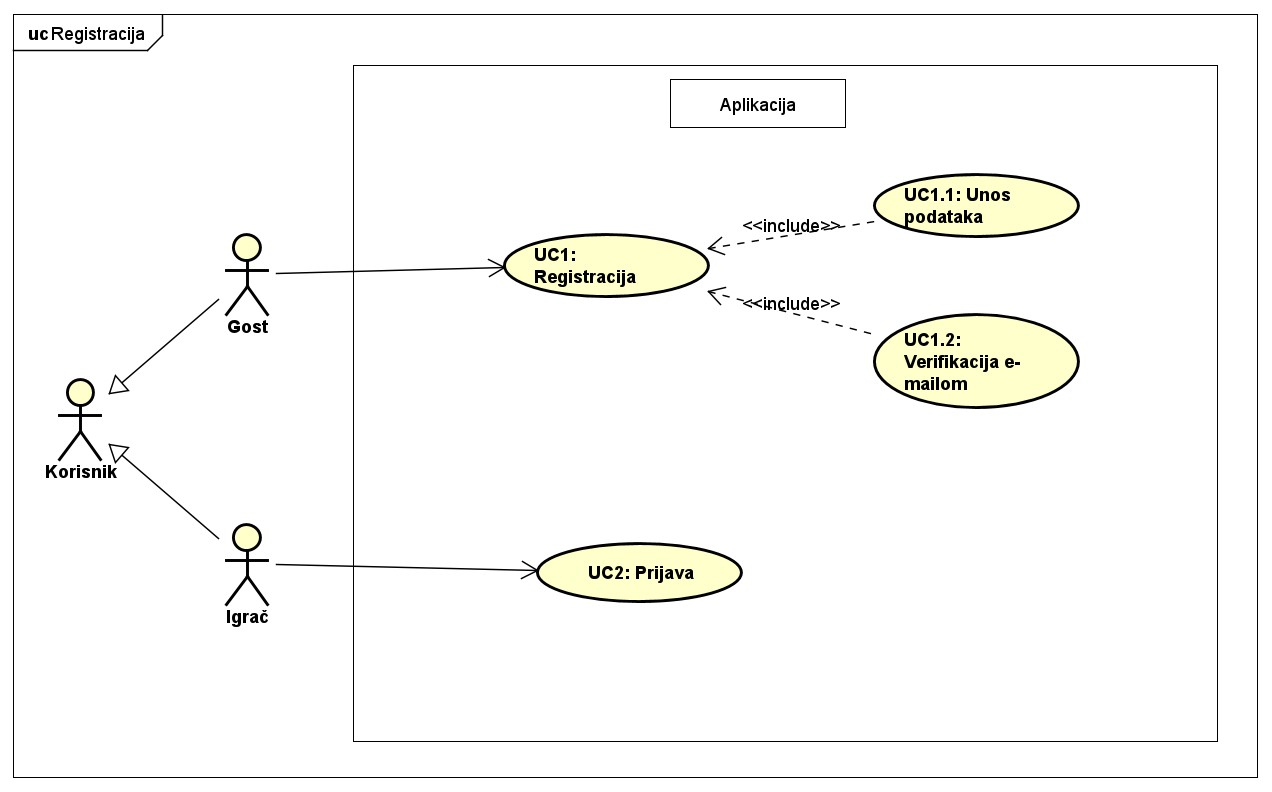
\includegraphics[width=\textwidth]{slike/UCRegistracija.png} %veličina u odnosu na širinu linije
			\caption{Prikaz UC za registraciju i prijavu}
			\label{fig:UCregistracija} %label mora biti drugaciji za svaku sliku
		\end{figure}
\pagebreak

		%unos slike
		\begin{figure}[H]
			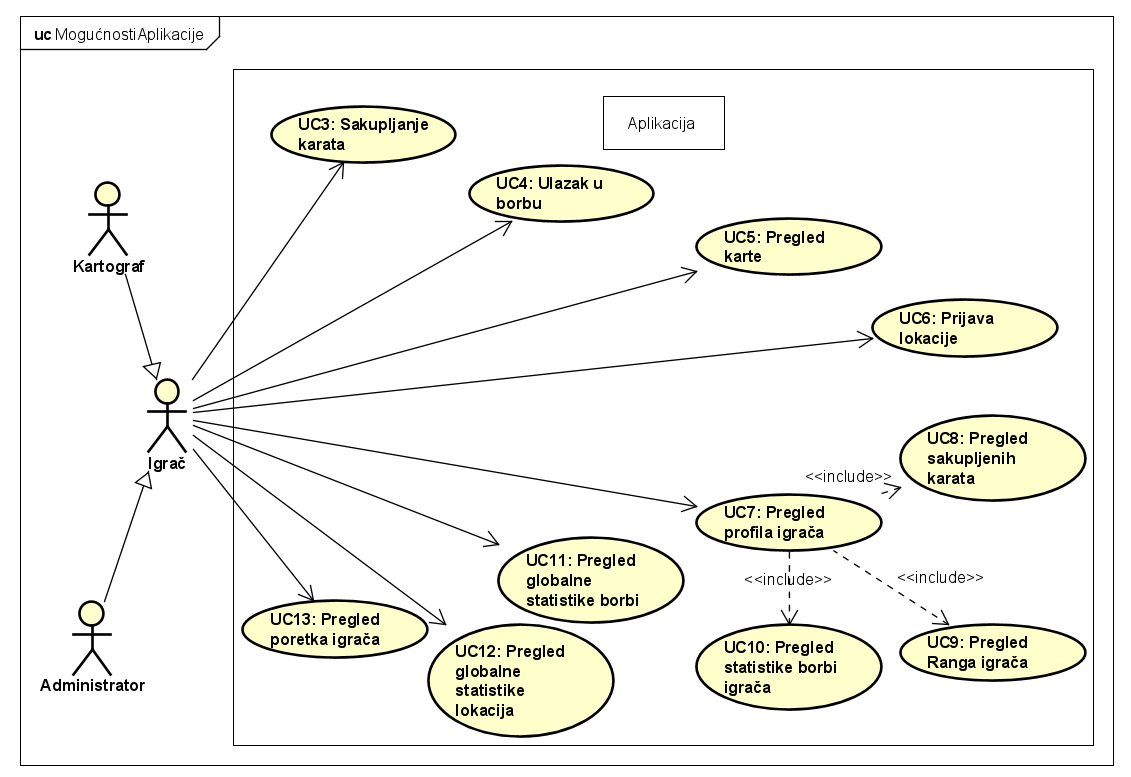
\includegraphics[width=\textwidth]{slike/UCMogucnostiAplikacije.png} %veličina u odnosu na širinu linije
			\caption{Prikaz UC za osnovne mogućnosti aplikacije dostupne igračima}
			\label{fig:UCmogucnostiAplikacije} %label mora biti drugaciji za svaku sliku
		\end{figure}
\pagebreak

		%unos slike
		\begin{figure}[H]
			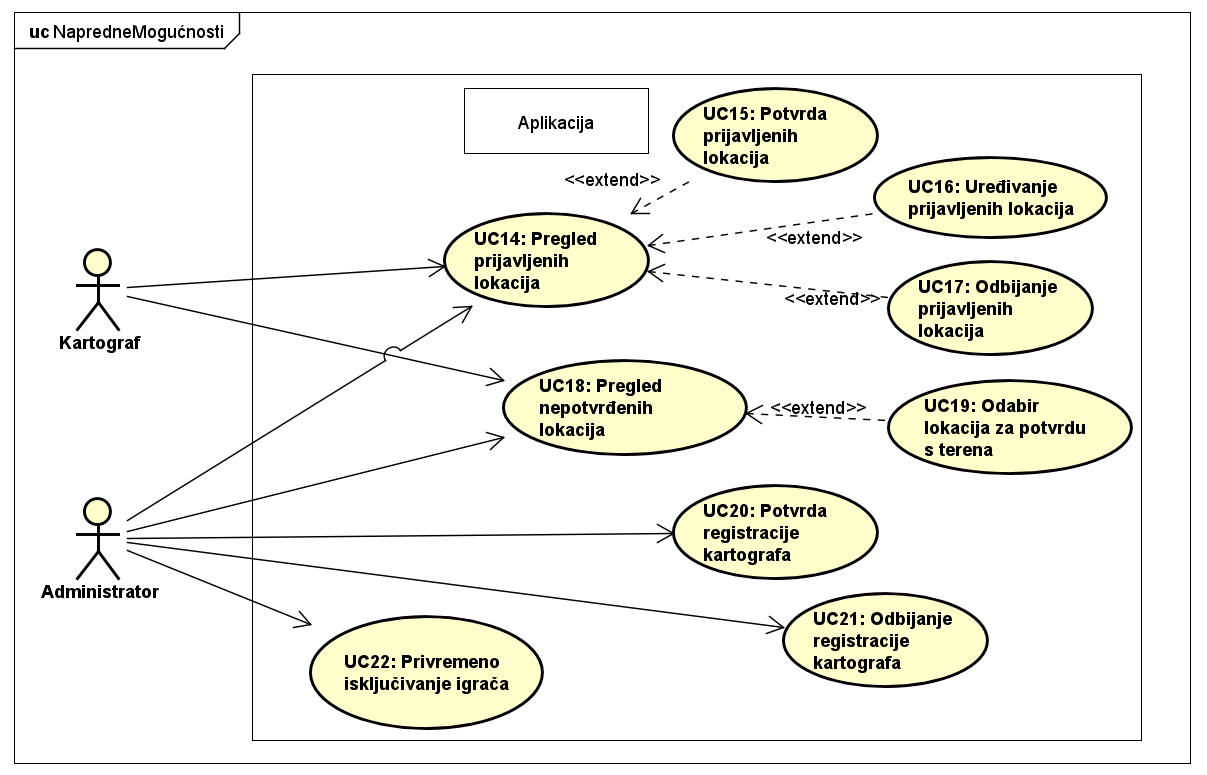
\includegraphics[width=\textwidth]{slike/UCNapredneMogucnosti.png} %veličina u odnosu na širinu linije
			\caption{Prikaz UC za napredne mogućnosti dostupne kartografima i administratorima}
			\label{fig:UCnapredneMogucnosti} %label mora biti drugaciji za svaku sliku
		\end{figure}
\pagebreak

%\textit{Prikazati odnos aktora i obrazaca uporabe odgovarajućim UML dijagramom. Nije nužno nacrtati sve na jednom dijagramu. Modelirati po razinama apstrakcije i skupovima srodnih funkcionalnosti.}
\eject		

\subsection{Sekvencijski dijagrami}

\textbf{\textit{dio 1. revizije}}\\

\noindent \textbf{Obrazac uporabe UC2 - Sakupljanje karata}
    Korisnik vidi na mapi kartu koju bi želio sakupiti. Korisnik odlazi do lokacije gdje može dobiti tu kartu. Dolaskom na lokaciju i odabirom "Skupi kartu lokacije" korisnik šalje zahtjev aplikaciji za sakupljanje karte. Aplikacija provjerava nalazi li se korisnik na navedenoj lokaciji, zatim dohvaća korisnikove podatke te provjerava ima li manje od 20 karata spremljenih. Ako je provjera zadovoljena, aplikacija daje šalje zahtjev bazi podataka da spremi korisniku kartu te lokacije. Konačno, aplikacija obavještava korisnika o uspješnom, odnosno neuspješnom sakupljanju karte.

		%unos slike
		\begin{figure}[H]
			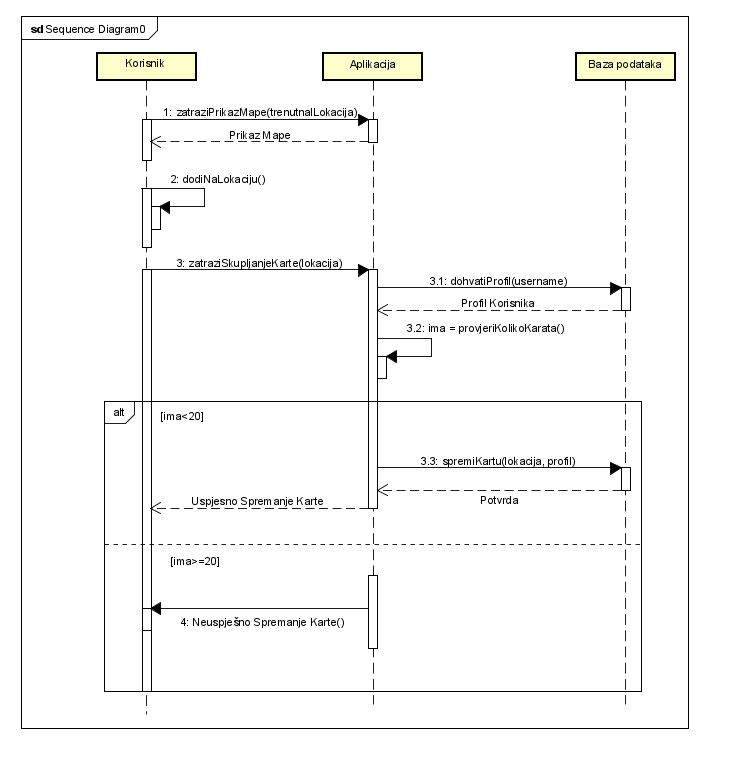
\includegraphics[width=\textwidth]{slike/SeqUC2.png} %veličina u odnosu na širinu linije
			\caption{Sekvencijski dijagram za UC2}
			\label{fig:promjene3} %label mora biti drugaciji za svaku sliku
		\end{figure}
\pagebreak

\noindent \textbf{Obrazac uporabe UC3 - Korisnik ulazi u borbu s njima}
    Korisnik želi otići u borbu. Korisnik je na stranici za prikaz ostalih korisnika u blizini. Korisnik odabire jedan profil i odabirom "Izazovi" šalje zahtjev aplikaciji za borbu protiv tog korisnika. Aplikacija šalje zahtjev drugome korisniku želi li ući u borbu s prethodnim korisnikom. Odgovor drugog korisnika aplikacija šalje natrag prvom korisniku. Ako je drugi korisnik prihvatio, aplikacija prikazuje stranicu za borbu korisnicima. Aplikacija šalje zahtjev bazi podataka za prikazom svih karata toga korisnika. Baza vraća podatke i aplikacija prikazuje korisniku njegove karte. Korisnik odabire kartu. Aplikacija uspoređuje jačinu karata i vraća rezultat korisnicima. Karti koju je korisnik koristio se smanjuje vrijednost za 10 posto. Ako drugi korisnik nije prihvatio borbu, aplikacija obaviještava korisnika o tome.
    
    		%unos slike
		\begin{figure}[H]
			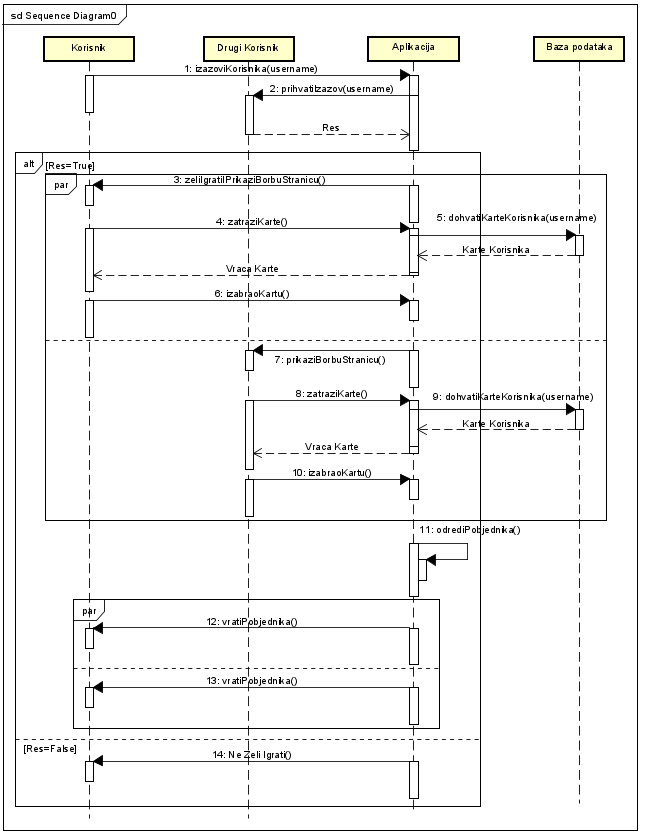
\includegraphics[width=\textwidth]{slike/SeqUC3.png} %veličina u odnosu na širinu linije
			\caption{Sekvencijski dijagram za UC3}
			\label{fig:promjene4} %label mora biti drugaciji za svaku sliku
		\end{figure}
\pagebreak

\noindent \textbf{Obrazac uporabe UC5 - Prijavljivanje željene lokacije}
    
    Korisnik se nalazi na mjestu koje je zanimljivo i želi ga dodati u aplikaciju. Korisnik odabire "Predloži lokaciju". Aplikacija dohvaća podatke o korisniku i provjerava ima li dovoljno iskustva. Ako nema dovoljno iskustva aplikacija obaviještava korisnika o tome. Ako ima dovoljno iskustva prikazuje stranicu u kojoj traži informacije o novoj lokaciji. Nakon što korisnik ispuni podatke i preda informacije, aplikacija šalje zahtjev bazi podataka da spremi navedenu lokaciju. Tu lokaciju baza sprema kao nepotvrđenu. Uz to baza sprema i podatke o korisniku koji je predložio lokaciju kako bi mu aplikacija kasnije mogla dati tu kartu.
    		%unos slike
		\begin{figure}[H]
			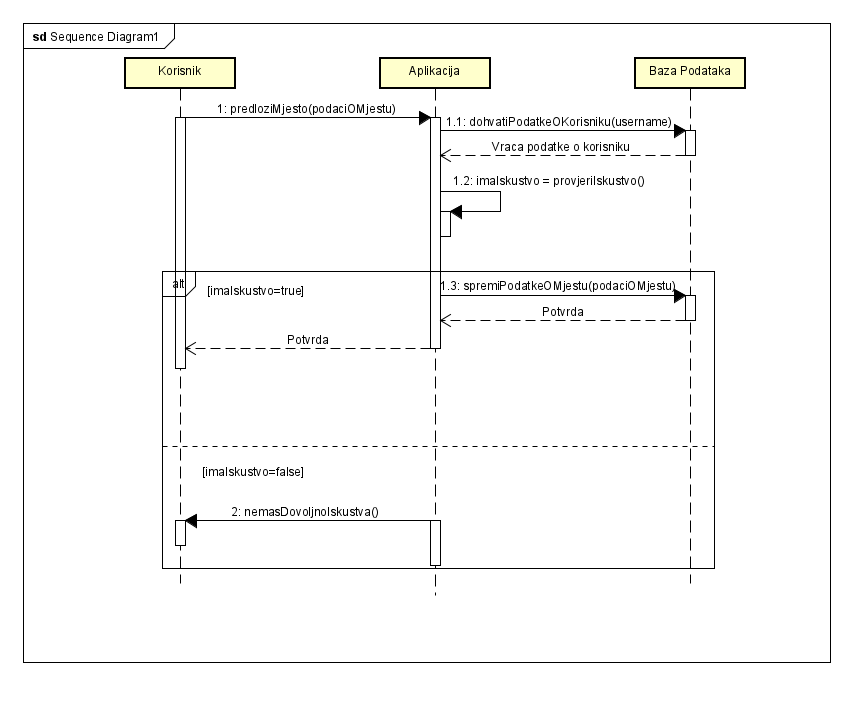
\includegraphics[width=\textwidth]{slike/SeqUC5.png} %veličina u odnosu na širinu linije
			\caption{Sekvencijski dijagram za UC3}
			\label{fig:promjene5} %label mora biti drugaciji za svaku sliku
		\end{figure}
\eject

\section{Ostali zahtjevi}

%\textbf{\textit{dio 1. revizije}}\\

%\textit{Nefunkcionalni zahtjevi i zahtjevi domene primjene dopunjuju funkcionalne zahtjeve. Oni opisuju \textbf{kako se sustav treba ponašati} i koja \textbf{ograničenja} treba poštivati (performanse, korisničko iskustvo, pouzdanost, standardi kvalitete, sigurnost...). Primjeri takvih zahtjeva u Vašem projektu mogu biti: podržani jezici korisničkog sučelja, vrijeme odziva, najveći mogući podržani broj korisnika, podržane web/mobilne platforme, razina zaštite (protokoli komunikacije, kriptiranje...)... Svaki takav zahtjev potrebno je navesti u jednoj ili dvije rečenice.}
	
		\begin{packed_item}
			\item Sustav treba omogućiti rad više korisnika u stvarnom vremenu
			\item Korisničko sučelje i sustav moraju podržavati hrvatsku abecedu (dijakritičke znakove) pri unosu i prikazu tekstualnog sadržaja
			\item Izvršavanje dijela programa u kojem se pristupa bazi podataka ne smije trajati duže od nekoliko sekundi
			\item Sustav treba biti implementiran kao web aplikacija koristeći objektno-orijentirane jezike
			\item Neispravno korištenje korisničkog sučelja ne smije narušiti funkcionalnost i rad sustava
			\item Sustav treba biti jednostavan za korištenje, korisnici se moraju znati koristiti sučeljem bez opširnih uputa
			\item Nadogradnja sustava ne smije narušavati postojeće funkcionalnosti sustava
			\item Veza s bazom podataka mora biti kvalitetno zaštićena, brza i otporna na vanjske greške
			\item Pristup sustavu mora biti omogućen iz javne mreže pomoću HTTPS
			\item Korisnik u svakom trenutku mora imati pristup GPS - u
			\item Moraju biti osigurana konzistentna prava i mogućnosti svim igračima podjednako
			\item Svaka nova registracija mora biti potvrđena putem e - mail adrese korisnika
			\item Svaka lokacija u aplikaciji mora korelirati stvarnoj lokaciji
			\item Sustav mora osigurati da svaka uloga ima samo njoj definirane ovlasti
			\item Baza podataka se kontinuirano mora osvježavati za obnovu podataka u slučaju prekida veze ili nestanka struje
		\end{packed_item}




